\def\linkdethi{} %Đường link cần dẫn tới
\anmaQR
%%%%%%%%%%%%%%%%%%%%%%%%
\def\toanlop{12}
\def\thoigian{90}
\def\namhoc{2025 - 2026}
\begin{dethi}
	{Bộ GD\&ĐT}
	{VTED ft KING EDU}
	{TDMT10}
	{Đề thi thử THPTQG 2026}
\end{dethi}
\caulc
\Opensolutionfile{ans}[ans/ansTN-Dung]
%%%=============EX_1=============%%%
\begin{ex}%[1D7H2-1]%[TDMT10]%[Bồ Văn Hậu]
	Cho hàm số $y=\mathrm{e}^{2x}$. Giá trị đạo hàm của hàm số tại $x=1\,000$ là
	\choice
	{$+\infty$}
	{$\mathrm{e}^{2\,000}$}
	{\True $2\cdot\mathrm{e}^{2\,000}$}
	{$2\cdot\mathrm{e}^{1\,000}$}
	\loigiai{
		Tập xác định $\mathscr{D}=\mathbb{R}$.\\
		Ta có $y=\mathrm{e}^{2x}$ suy ra $y'=\left(\mathrm{e}^{2x}\right)'=\mathrm{e}^{2x}\cdot (2x)'=2\cdot\mathrm{e}^{2x}$.\\
		Suy ra giá trị đạo hàm của hàm số tại $x=1\,000$ là $y'(1\,000)=2\cdot\mathrm{e}^{2\,000}$.
	}
\end{ex}
%%%=============================%%%

%%%=============EX_2=============%%%
\begin{ex}%[1D2N3-4]%[TDMT10]%[Đình Nguyên]
	Cho cấp số nhân $(u_n)$ có số hạng đầu bằng $3$ và công bội bằng $2$. Số hạng thứ $3$ là
	\choice
	{\True $12$}
	{$24$}
	{$9$}
	{$7$}
	\loigiai{
		Ta có số hạng tổng quát của cấp số nhân là $u_n = u_1 \cdot q^{n-1}$.\\
		Suy ra $u_3 = u_1 \cdot q^2 = 3 \cdot 2^2 = 12$.
	}
\end{ex}
%%%=============================%%%

%%%=============EX_3=============%%%
\begin{ex}%[1D6H4-4]%[TDMT10]%[Trần Văn Thiện]
	Tập nghiệm của phương trình $\log_{x-4}\left(x^2-7x+12\right)=\log_{x-4}\left(x-3\right)$ là
	\choice
	{$\mathrm{S}=\{3;5\}$}
	{$\mathrm{S}=\{5\}$}
	{ $\mathrm{S}=\{3\}$}
	{\True$\mathrm{S}=\varnothing$}
	\loigiai{
		Điều kiện $\heva{&x-4>0\\ &x-4\neq 1\\&x^2-7x+12>0\\&x-3>0}\Leftrightarrow \heva{&x>4\\
			&x\neq 5 .}$ \\
		Khi đó phương trình cho trở thành $ x^2-7x+12=x-3\Leftrightarrow x^2-8x+15=0\Leftrightarrow \hoac{&x=3\\ &x=5.}$\\
		Đối chiếu điều kiện, phương trình cho vô nghiệm.
	}
\end{ex}
%%%=============================%%%

%%%=============EX_4=============%%%
\begin{ex}%[1H8H7-2]%[TDMT10]%[Mui Doan]
	Cho hình chóp $S.ABC$ có đáy là tam giác đều cạnh $a$, cạnh bên $SA$ vuông góc với đáy, góc tạo bởi đường thẳng $SB$ với đáy bằng $60^\circ$. Thể tích khối chóp $S.ABC$ bằng
	\choice
	{\True $\dfrac{a^3}{4}$}
	{$\dfrac{3a^3}{4}$}
	{$\dfrac{a^3\sqrt{3}}{6}$}
	{$\dfrac{a^3\sqrt{2}}{4}$}
	\loigiai{
		\immini{
			Vì $SA \perp (ABC)$ nên $SA$ là chiều cao của hình chóp.\\
			$SB$ có hình chiếu lên $(ABC)$ là $AB$.\\
			Suy ra $\left(SB,(ABC)\right)=(SB,AB)=\widehat{SBA}=60^\circ$.\\
			Tam giác $SAB$ vuông tại $A$ có
			\[
			\tan 60^\circ=\dfrac{SA}{AB}\Rightarrow SA=AB\cdot \tan 60^\circ=a\sqrt{3}.
			\]
			Diện tích đáy $S_{ABC}=\dfrac{a^2\sqrt3}{4}$.\\
			Thể tích khối chóp
			\[
			V=\dfrac{1}{3}S_{ABC}\cdot SA
			=\dfrac{1}{3}\cdot\dfrac{a^2\sqrt3}{4}\cdot a\sqrt{3}
			=\dfrac{a^3}{4}.
			\]
		}
		{
			\begin{tikzpicture}[declare function={goc=-45; a=5; b=0.45*a; h=4;}, line join=round, line cap=round, >=stealth, font=\footnotesize]
				\path 
				(0,0) coordinate (A)--+(0,h) coordinate (S)
				(a,0) coordinate (C)
				(goc:b) coordinate (B);
				
				\path pic[angle radius=3mm,draw] {right angle = S--A--C};
				\path pic[angle radius=3mm,draw] {right angle = S--A--B};
				\path pic[draw,"$60^\circ$",angle eccentricity=1.6, angle radius=0.8cm] {angle =S--B--A};
				
				\draw[dashed] (A)--(C);
				\draw (S)--(B) (S)--(A)--(B)--(C)--cycle;
				
				\foreach \x/\goc in {S/90,A/240,C/-60,B/-90} {
					\filldraw (\x) circle (1pt) node[shift={(\goc:3mm)}]{$\x$};
				}
			\end{tikzpicture}
		}
	}
\end{ex}
%%%=============================%%%

%%%=============EX_5=============%%%
\begin{ex}%[2H2H1-2]%[TDMT10]%[Nguyễn Trí Minh Tuấn]
	Trong không gian $Oxyz$, cho hai vectơ $\overrightarrow{u}=(2;1;-1)$ và $\overrightarrow{v}=(1;3;1)$. Tọa độ của vectơ $\overrightarrow{u}+2\overrightarrow{v}$ tương ứng là
	\choice
	{$(3;4;0)$}
	{$(1;-2;-2)$}
	{\True $(4;7;1)$}
	{$(5;5;-1)$}
	\loigiai{
		Ta có $\overrightarrow{u}+2\overrightarrow{v}=(2;1;-1)+2(1;3;1)=(2;1;-1)+(2;6;2)=(4;7;1)$.
	}
\end{ex}
%%%=============================%%%

%%%=============EX_6=============%%%
\begin{ex}%[TDMT10]%[2D1N3-2]%[Huỳnh Quốc Đạt]
	Cho hàm số $y=f(x)$ có bảng biến thiên như hình vẽ bên dưới. Giá trị nhỏ nhất của hàm số $f(x)$ trên $(-\infty;0)$ bằng
	\begin{center}
		
\begin{tikzpicture}
			\tkzTabInit[lgt=1.5, espcl=2.5]{$x$/1,$f(x)$/3}
			{$-\infty$,$-2$,$0$,$3$,$+\infty$}
			\tkzTabVar{+/$+\infty$,-/$1$,+D+/$+\infty$/$+\infty$,-/$2$,+/$+\infty$}
		\end{tikzpicture}
	\end{center}
	\choice
	{$2$}
	{\True $1$}
	{$-\infty$}
	{không tồn tại}
	\loigiai{
		Dựa vào bảng biến thiên ta có $\min\limits_{(-\infty;0)}f(x)=f(-2)=1$.
	}
\end{ex}
%%%=============================%%%

%%%=============EX_7=============%%%
\begin{ex}%[2D1H2-1]%[TDMT10]%[Chu Ha]
	Hàm số $f(x)=x^5-5x$ có điểm cực tiểu là
	\choice
	{$x=-1$}
	{\True $x=1$}
	{$y=4$}
	{$y=-4$}
	\loigiai{
		Ta có $f'(x)=5x^4-5$, khi đó $f'(x)=0 \Leftrightarrow 5x^4-5=0 \Leftrightarrow\hoac{&x=1\\&x=-1.}$\\
		Ta có bảng biến thiên
		\begin{center}
			
\begin{tikzpicture}[font=\normalsize, >=stealth]
				\tkzTabInit[lgt=1.2,espcl=2.5]
				{$x$/1,$f'(x)$/1,$f(x)$/2}
				{$-\infty$,$-1$,$1$,$+\infty$}
				\tkzTabLine{,+,0,-,0,+,}
				\tkzTabVar{-/$-\infty$,+/$4$,-/$-4$,+/$+\infty$}
			\end{tikzpicture}
		\end{center}
		Dựa vào bảng biến thiên ta kết luận được hàm số có điểm cực tiểu là $x=1$.
	}
\end{ex}
%%%=============================%%%

%%%=============EX_8=============%%%
\begin{ex}%[2D1N4-1]%[TDMT10]%[Nguyễn Tấn Linh]
	Đồ thị của hàm số $y=\dfrac{x-5}{x+2}$
	\choice
	{không có tiệm cận ngang}
	{không có trục đối xứng}
	{có hai điểm cực trị}
	{\True có hai đường tiệm cận}
	\loigiai{
		Tập xác định $\mathscr{D}=\mathbb{R}\setminus\{-2\}$.\\
		Ta có $\lim\limits_{x \to \pm \infty} y = \lim\limits_{x \to \pm \infty} \dfrac{x-5}{x+2} = 1$ nên đồ thị hàm số có đường tiệm cận ngang $y=1$.\\
		Lại có $\lim\limits_{x \to -2^+} y = -\infty$ và $\lim\limits_{x \to -2^-} y = +\infty$ nên đồ thị hàm số có đường tiệm cận đứng $x=-2$.\\
		Vậy đồ thị hàm số đã cho có tất cả hai đường tiệm cận (một đứng, một ngang).
	}
\end{ex}
%%%=============================%%%

%%%=============EX_9=============%%%
\begin{ex}%[2H2H1-3]%[TDMT10]%[Lê Phúc]
	Cho hình chóp đều $S.ABCD$ có đáy $ABCD$ là hình vuông cạnh bằng $6$ và cạnh bên $SA=8$. Giá trị của tích vô hướng $\overrightarrow{SA}\cdot\overrightarrow{CD}$ bằng
	\choice
	{\True $18$}
	{$-18$}
	{$24$}
	{$-24$}
	\loigiai{
		\immini{
			Gọi $H$ là trung điểm của $AB$.\\
			Do $\triangle SAB$ cân tại $S$ nên $SH\perp AB$ (trung tuyến đồng thời là đường cao).\\
			Ta có 
			\allowdisplaybreaks
			\begin{align*}
				\overrightarrow{SA}\cdot\overrightarrow{CD} &= \overrightarrow{SA}\cdot\overrightarrow{BA}=\overrightarrow{AS}\cdot\overrightarrow{AB}\\
				&= AS\cdot AB\cdot \cos\widehat{SAB}=AS\cdot AB\cdot \dfrac{AH}{SA}\\
				&= AB\cdot AH = 6\cdot 3=18.
			\end{align*}
		}{
			\begin{tikzpicture}[line join=round, line cap=round, >=stealth, font=\footnotesize, scale=0.7]
				\coordinate (A) at (0,0);
				\coordinate (B) at (2,-2);
				\coordinate (D) at (5,0);
				\coordinate (C) at ($(B)+(D)-(A)$);
				\coordinate (O) at ($(A)!0.5!(C)$);
				\coordinate (H) at ($(A)!0.5!(B)$);
				\coordinate (S) at ($(O)+(0,7)$);
				
				\draw (S)--(A) (S)--(B) (S)--(C) (A)--(B) (B)--(C) (S)--(H);
				\draw[dashed] (A)--(C) (A)--(D) (C)--(D) (S)--(D) (S)--(O) (B)--(D);
				
				\path pic[draw,thin,angle radius=2mm] {right angle = S--O--D};
				\path pic[draw,thin,angle radius=2mm] {right angle = S--O--A};
				\path pic[draw,thin,angle radius=2mm] {right angle = S--H--A};
				
				\foreach \i/\g in {S/90, A/180, B/-90, C/-90, D/0, O/-90, H/180} {
					\filldraw (\i) circle (1pt) node[shift={(\g:3mm)}]{$\i$};
				}
			\end{tikzpicture}
	}}
\end{ex}
%%%=============================%%%

%%%=============EX_10=============%%%
\begin{ex}%[2H5H2-5]%[TDMTD010]%[Phạm Hải Dương]
	Trong không gian $Oxyz$, cho hai điểm $A(2;3;-1)$ và $B(4;-1;3)$. Giao điểm của $AB$ và mặt phẳng $(Oxy)$ có toạ độ là
	\choice
	{$\left(-\dfrac{5}{2}; 2; 0\right)$}
	{$\left(0; 2; \dfrac{3}{2}\right)$}
	{\True $\left(\dfrac{5}{2}; 2; 0\right)$}
	{$\left(\dfrac{3}{2}; -4; 0\right)$}
	\loigiai{
		Ta có $\overrightarrow{AB}=(2; -4; 4)$. Phương trình tham số của đường thẳng $AB$ là $\heva{&x=2+2t \\&y=3-4t \\&z=-1 + 4t.}$ \\
		Giao điểm của đường thẳng $AB$ và mặt phẳng $(Oxy)$ ứng với $z = 0 \Rightarrow -1 + 4t = 0 \Rightarrow t = \dfrac{1}{4}$.\\
		Thay $t = \dfrac{1}{4}$ vào phương trình đường thẳng $AB$ ta được:
		$x = 2 + 2 \cdot \dfrac{1}{4} = \dfrac{5}{2}$; $y = 3 - 4 \cdot \dfrac{1}{4} = 2$.\\
		Vậy toạ độ giao điểm là $\left(\dfrac{5}{2}; 2; 0\right)$.
	}
\end{ex}
%%%=============================%%%

%%%=============EX_11=============%%%
\begin{ex}%[2H2H1-2]%[TDMT10]%[Huỳnh Trí Thiện]
	Cho hình hộp $ABCD.MNPQ$. Khi đó nhận xét đúng là
	\choice
	{$\overrightarrow{AB} + \overrightarrow{NP} + \overrightarrow{NB} = \overrightarrow{AP}$}
	{\True $\overrightarrow{AB} + \overrightarrow{NP} + \overrightarrow{DQ} = \overrightarrow{AP}$}
	{$\overrightarrow{AB} + \overrightarrow{BP} + \overrightarrow{MA} = \overrightarrow{AP}$}
	{$\overrightarrow{AC} + \overrightarrow{CN} + \overrightarrow{BP} = \overrightarrow{AP}$}
	\loigiai{
		\immini{
			Theo tính chất của hình hộp, ta có các cặp vectơ bằng nhau: $\overrightarrow{NP} = \overrightarrow{BC} = \overrightarrow{AD}$ và $\overrightarrow{DQ} = \overrightarrow{AM}$.\\
			Khi đó
			\[ \overrightarrow{AB} + \overrightarrow{NP} + \overrightarrow{DQ} = \overrightarrow{AB} + \overrightarrow{AD} + \overrightarrow{AM}. \]
			Áp dụng quy tắc hình hộp ta có
			\[ \overrightarrow{AB} + \overrightarrow{AD} + \overrightarrow{AM} = \overrightarrow{AP}. \]
			Vậy đẳng thức đúng là $\overrightarrow{AB} + \overrightarrow{NP} + \overrightarrow{DQ} = \overrightarrow{AP}$.
		}{
			\begin{tikzpicture}[scale=0.6, line join=round, line cap=round, >=stealth, font=\footnotesize]
				\coordinate (A) at (0,0);
				\coordinate (B) at (4,0);
				\coordinate (D) at (2.5,1.5);
				\coordinate (M) at (1.5,4); 
				
				\coordinate (C) at ($(B)+(D)-(A)$);
				\coordinate (N) at ($(B)+(M)-(A)$); 
				\coordinate (Q) at ($(D)+(M)-(A)$); 
				\coordinate (P) at ($(C)+(M)-(A)$); 
				
				\draw[dashed] (D)--(A) (D)--(C) (D)--(Q);
				\draw (A)--(B)--(C)--(P)--(Q)--(M)--cycle;
				\draw (B)--(N)--(P) (N)--(M);
				
				\foreach \x/\g in {A/-135, B/-90, C/-45, D/135, M/135, N/90, P/0, Q/90} {
					\filldraw (\x) circle (1.5pt) node[shift={(\g:3mm)}]{$\x$};
				}
			\end{tikzpicture}
	}}
\end{ex}
%%%=============================%%%

%%%=============EX_12=============%%%
\begin{ex}%[2D3H1-2]%[TDMT10]%[Nguyễn Sơn Thành]
	Cho mẫu số liệu ghép nhóm $M$ gồm có $8$ nhóm có độ dài bằng nhau, đầu mút trái của nhóm thứ $3$ và đầu mút phải của nhóm thứ $5$ lần lượt là $4$ và $16$. Hãy xác định khoảng biến thiên của mẫu số liệu $M$.
	\choice
	{\True $32$}
	{$28$}
	{$16$}
	{$24$}
	\loigiai{
		\begin{itemize}
			\item Gọi $l$ là độ dài của mỗi nhóm trong mẫu số liệu $M$.
			\item Theo đề bài, từ đầu mút trái của nhóm thứ $3$ đến đầu mút phải của nhóm thứ $5$ bao gồm $3$ nhóm liên tiếp (nhóm $3$, $4$, $5$).
			\item Khoảng cách này được tính bằng $3l = 16 - 4 = 12 \Rightarrow l = 4$.
			\item Khoảng biến thiên của mẫu số liệu ghép nhóm $R$ được tính bằng hiệu giữa đầu mút phải của nhóm cuối cùng và đầu mút trái của nhóm đầu tiên.
			\item Vì có $8$ nhóm với độ dài bằng nhau nên $R = 8 \cdot l = 8 \cdot 4 = 32$.
		\end{itemize}
	}
\end{ex}
%%%=============================%%%
\Closesolutionfile{ans}

\cauds
\Opensolutionfile{ans}[ans/ansTN-DungSai]
%%%=============EX_13=============%%%
\begin{ex}%[2H2H2-2]%[TDM31]%[Nguyễn Văn Sang]
	Trong không gian $Oxyz$, cho ba điểm $A(2;2;0)$, $B(0;0;1)$, $C(2;-2;3)$.
	\choiceTF[t]
	{\True $AC = 5$}
	{$\cos\left(\overrightarrow{AB}, \overrightarrow{AC}\right) = \dfrac{2}{3}$}
	{Toạ độ trọng tâm của tam giác $ABC$ là $(4;0;4)$}
	{\True Gọi $I$ là tâm đường tròn nội tiếp tam giác $ABC$. Khi đó ta có $OI = 1{,}66$ \textit{(làm tròn kết quả đến hàng phần trăm)}}
	\loigiai{
		Ta có $\overrightarrow{AB} = (-2;-2;1)$, $\overrightarrow{AC} = (0;-4;3)$, $\overrightarrow{BC} = (2;-2;2)$.\\
		Suy ra $AB = \sqrt{(-2)^2 + (-2)^2 + 1^2} = 3$, $AC = \sqrt{0^2 + (-4)^2 + 3^2} = 5$, $BC = \sqrt{4+4+4} = 2\sqrt{3}$.
		\begin{itemchoice}
			\itemch $AC = \sqrt{0^2 + (-4)^2 + 3^2} = \sqrt{25} = 5$.
			\itemch Ta có
			$\cos\left(\overrightarrow{AB}, \overrightarrow{AC}\right) = \dfrac{\overrightarrow{AB} \cdot \overrightarrow{AC}}{|\overrightarrow{AB}| \cdot |\overrightarrow{AC}|} = \dfrac{(-2) \cdot 0 + (-2) \cdot (-4) + 1 \cdot 3}{3 \cdot 5} = \dfrac{11}{15} \neq \dfrac{2}{3}$.
			\itemch Trọng tâm $G$ của tam giác $ABC$ có toạ độ
			\[G = \left(\dfrac{x_A + x_B + x_C}{3}; \dfrac{y_A + y_B + y_C}{3}; \dfrac{z_A + z_B + z_C}{3}\right) = \left(\dfrac{2+0+2}{3}; \dfrac{2+0-2}{3}; \dfrac{0+1+3}{3}\right) = \left(\dfrac{4}{3}; 0; \dfrac{4}{3}\right).\]
			Vậy toạ độ trọng tâm là $\left(\dfrac{4}{3}; 0; \dfrac{4}{3}\right) \neq (4;0;4)$.
			\itemch Tâm đường tròn nội tiếp $I$ của tam giác $ABC$ có toạ độ
			\[I = \dfrac{a \cdot A + b \cdot B + c \cdot C}{a + b + c}\]
			với $a = BC = 2\sqrt{3}$, $b = CA = 5$, $c = AB = 3$.\\
			Ta có
			\allowdisplaybreaks
			\begin{align*}
				x_I &= \dfrac{2\sqrt{3} \cdot 2 + 5 \cdot 0 + 3 \cdot 2}{2\sqrt{3} + 5 + 3} = \dfrac{4\sqrt{3} + 6}{8 + 2\sqrt{3}} \approx 1{,}18\\
				y_I &= \dfrac{2\sqrt{3} \cdot 2 + 5 \cdot 0 + 3 \cdot (-2)}{2\sqrt{3} + 5 + 3} = \dfrac{4\sqrt{3} - 6}{8 + 2\sqrt{3}} \approx 0{,}09\\
				z_I &= \dfrac{2\sqrt{3} \cdot 0 + 5 \cdot 1 + 3 \cdot 3}{2\sqrt{3} + 5 + 3} = \dfrac{14}{8 + 2\sqrt{3}} \approx 1{,}27
			\end{align*}
			Suy ra $OI = \sqrt{x_I^2 + y_I^2 + z_I^2} \approx \sqrt{1{,}18^2 + 0{,}09^2 + 1{,}27^2} \approx 1{,}66$.
		\end{itemchoice}
	}
\end{ex}
%%%=============================%%%

%%%=============EX_14=============%%%
\begin{ex}%[2D1V4-1]%[TDMT08]%[Vũ Hồng Toàn]
	Cho hàm số $y=f(x)=\dfrac{3x+3}{x^2-4x+3}$ có đồ thị $(C)$.
	\choiceTF[t]
	{\True Đồ thị $(C)$ có đúng $3$ đường tiệm cận}
	{\True Đồ thị của hàm số $y=(x-1)f(x)$ có đúng $2$ đường tiệm cận}
	{Đồ thị hàm số $y=(x^2-x)f(x)$ có tâm đối xứng là $I(2;1)$}
	{\True Có đúng $5$ điểm có tọa độ nguyên nằm trên đồ thị $(C)$}
	\loigiai{
		Hàm số đã cho xác định khi $x^2-4x+3\ne 0\Rightarrow\heva{&x\ne 1\\&x\ne 3.}$\\
		Vậy tập xác định của hàm số là $\mathscr{D} = \mathbb{R} \setminus \{1; 3\}$.
		\begin{itemchoice}
			\itemch Ta có
			\begin{itemize}
				\item $\lim\limits_{x \to 1^+} \dfrac{3x+3}{(x-1)(x-3)} = -\infty$. Do đó $x=1$ là một tiệm cận đứng.
				\item $\lim\limits_{x \to 3^+} \dfrac{3x+3}{(x-1)(x-3)} = +\infty$. Do đó, $x=3$ là một tiệm cận đứng.
				\item $\lim\limits_{x \to \pm\infty} \dfrac{3x+3}{x^2-4x+3} = 0$. Do đó, $y=0$ là một tiệm cận ngang.
			\end{itemize}
			Vậy, hàm số đã cho có $3$ đường tiệm cận.
			\itemch Xét hàm số $y = (x-1)f(x) =(x-1) \cdot \dfrac{3x+3}{(x-1)(x-3)}= \dfrac{3x+3}{x-3}$ với $x \ne 1$.\\
			Tập xác định $\mathscr{D} = \mathbb{R} \setminus \{3\}$.
			\begin{itemize}
				\item $\lim\limits_{x \to 3^+} \dfrac{3x+3}{x-3} = +\infty$. Do đó, $x=3$ là một tiệm cận đứng.
				\item $\lim\limits_{x \to \pm\infty} \dfrac{3x+3}{x-3} = 3$. Do đó, $y=3$ là một tiệm cận ngang.
			\end{itemize}
			Vậy hàm số $y = (x-1)f(x)$ có $2$ đường tiệm cận.
			\itemch Xét hàm số\\ $y = (x^2-x)f(x) =x(x-1) \cdot \dfrac{3x+3}{(x-1)(x-3)}= \dfrac{3x^2+3x}{x-3}=3x+12 + \dfrac{36}{x-3}$ với $x \ne 1$.\\
			Tập xác định $\mathscr{D} = \mathbb{R} \setminus \{3\}$.\\
			Đồ thị hàm số đã cho có tiệm cận đứng là $x=3$ và tiệm cận xiên là $y=3x+12$.\\
			Do đó có tâm đối xứng là $I(3;21)$.
			\itemch Vì $x\in\mathbb{Z}\Rightarrow(x-3)\in\mathbb{Z}$ nên
			$(x-3)f(x) = \dfrac{3x+3}{x-1} = 3+ \dfrac{6}{x-1}\in\mathbb{Z}\Rightarrow \dfrac{6}{x-1}\in\mathbb{Z}$.\\
			Xét $x-1$ là ước của $6$ thì $x-1 \in \{-6; -3; -2;-1; 1;2;3;6\}$.\\ Khi đó
			\begin{center}
				\begin{tabular}{|c|c|c|c|}
					\hline
					$x-1 = -6$	& $x=-5$ & $f(-5)=-\frac{1}{4}$ & loại \\
					\hline
					$x-1 = -3$	& $x=-2$ & $f(-2)=-\frac{1}{5}$ & loại \\
					\hline
					$x-1 = -2$	& $x=-1$ & $f(-1)=0$ & nhận \\
					\hline
					$x-1 = -1$	& $x=0$ & $f(0)=-3$ & nhận \\
					\hline
					$x-1 = 1$	& $x=2$ & $f(2)=-9$ & nhận \\
					\hline
					$x-1 = 2$	& $x=3\notin \mathscr{D}$ & & loại \\
					\hline
					$x-1 = 3$	& $x=4$ & $f(4)=5$ & nhận \\
					\hline
					$x-1 = 6$	& $x=7$ & $f(7)=1$ & nhận \\
					\hline
				\end{tabular}
			\end{center}
			Vậy có $5$ điểm nguyên thuộc $(C)$.
		\end{itemchoice}
	}
\end{ex}
%%%=============================%%%

%%%=============EX_15=============%%%
\begin{ex}%[2D1H5-8]%[TDMTD10]%[Dương Công Tạo]
	Khối lượng $x$ (kg) của một loại hoa quả mà cửa hàng bán được trong một ngày phụ thuộc vào giá bán $p$ (nghìn đồng/kg) theo hàm cầu $p=60-\dfrac{1}{5}x$.
	\choiceTF[t]
	{\True Giá bán khi cửa hàng bán được $25$\,kg hoa quả là $55$ nghìn đồng/kg}
	{Doanh thu của cửa hàng khi bán được $60$\,kg hoa quả là $3{,}18$ triệu đồng}
	{\True Để doanh thu là lớn nhất thì cửa hàng nên bán $150$\,kg hoa quả loại đang xét}
	{\True Nhận thấy khi bán hàng càng nhiều thì doanh thu cửa hàng sẽ ngày càng sụt giảm, cửa hàng quyết định điều chỉnh giá bán như sau: Giữ nguyên mức giá $p(x)=60-0{,}2x$ khi bán được hết $160$\,kg hoa quả. Sau đó, mỗi kg hoa quả sẽ được bán với giá $26$ nghìn đồng cho đến khi hết hàng. Khi đó, doanh thu của cửa hàng khi bán được $b$ (kg) hoa quả (với $b > 160$) là $26b+320$ (nghìn đồng)}
	\loigiai{
		\begin{itemchoice}
			\itemch Giá bán khi cửa hàng bán được $25$\,kg hoa quả là $p(25)=60-\dfrac{1}{5}\cdot 25=55$ nghìn đồng/kg.
			\itemch Doanh thu của cửa hàng khi bán được $x$\,kg hoa quả là 
			\[L(x)=x\cdot p(x)=x\cdot\left(60-\dfrac{1}{5}x\right)=60x-\dfrac{1}{5}x^2\text{ (nghìn đồng)}.\]
			Doanh thu của cửa hàng khi bán được $60$\,kg hoa quả là 
			\[L(60)=60\cdot 60-\dfrac{1}{5}60^2=2\,880\text{ (nghìn đồng) }=2{,}88\text{ (triệu đồng)}.\]
			\itemch Ta có $L'(x)=60-\dfrac{2}{5}x$; $L'(x)=0\Leftrightarrow x=150$.\\
			Bảng biến thiên
			\begin{center}
				
\begin{tikzpicture}[>=stealth]
					\tkzTabInit[nocadre=false,lgt=1.5,espcl=3,deltacl=0.6]{$x$/.7 ,$L'(x)$/.7,$L(x)$/2}
					{$0$ , $150$ , $+\infty$}
					\tkzTabLine{ , + , $0$ , - , }
					\tkzTabVar{-/$0$ , +/$4\,500$ , -/$-\infty$ }
				\end{tikzpicture}
			\end{center}
			Vậy, doanh thu lớn nhất là $4{,}5$ (triệu đồng) khi cửa hàng bán $150$\,kg hoa quả.
			\itemch Doanh thu của cửa hàng
			\begin{itemize}
				\item Khi bán $160$\,kg hoa quả đầu tiên là $160\cdot(60-0{,}2\cdot 160)=4\,480$ (nghìn đồng).
				\item Khi bán $b-160$\,kg hoa quả còn lại là $(b-160)\cdot 26$ (nghìn đồng).
			\end{itemize}
			Do đó, tổng doanh thu của cửa hàng khi bán được $b$ (kg) hoa quả (với $b > 160$) là 
			\[4\,480+(b-160)\cdot 26=26b+320\text{ (nghìn đồng)}.\]
		\end{itemchoice}
	}
\end{ex}
%%%=============================%%%

%%%=============EX_16=============%%%
\begin{ex}%[2H2V1-4]%[TDMT10]%[Văn Minh Thoại]
	\immini[thm]{
		Trong không gian, cho bốn sợi dây buộc với nhau tại nút $I$. Nút $I$ được cân bằng bởi $4$ lực dọc theo $4$ sợi dây thứ $1$, thứ $2$, thứ $3$, thứ $4$ lần lượt là $\overrightarrow{F}_1$, $\overrightarrow{F}_2$, $\overrightarrow{F}_3$, $\overrightarrow{F}_4$. Biết rằng $\left|\overrightarrow{F}_1\right|=120\mathrm{\,N}$, $\left|\overrightarrow{F}_2\right|=160\mathrm{\,N}$, $\left(\overrightarrow{F}_1,\overrightarrow{F}_2\right)=90^\circ$, $\left(\overrightarrow{F}_1,\overrightarrow{F}_3\right)=60^\circ$.
	}{
		\begin{tikzpicture}[line join=round, line cap=round, >=stealth, font=\footnotesize, scale=0.8]
			\path
			(0,0) coordinate (I)
			(1.5,-0.5) coordinate (F1)
			(-0.3,1.2) coordinate (F2)
			(2,0) coordinate (F3)
			(-1,-0.8) coordinate (F4);
			
			\draw[red,thick] (I) -- ($(I)!2.5!(F1)$)
			(I) -- ($(I)!2.2!(F2)$)
			(I) -- ($(I)!1.8!(F3)$)
			(I) -- ($(I)!2.5!(F4)$);
			
			\draw[blue,thick,->] (I) -- (F1) node[below right] {$\overrightarrow{F}_1$}
			(I) -- (F2) node[above right] {$\overrightarrow{F}_2$}
			(I) -- (F3) node[above] {$\overrightarrow{F}_3$}
			(I) -- (F4) node[above left] {$\overrightarrow{F}_4$};
			
			\filldraw (I) circle (2pt) node[left] {$I$};
		\end{tikzpicture}
	}
	\choiceTF[t]
	{\True $\overrightarrow{F}_1+\overrightarrow{F}_2+\overrightarrow{F}_3+\overrightarrow{F}_4=\overrightarrow{0}$}
	{\True $\left|\overrightarrow{F}_3+\overrightarrow{F}_4\right|=200\mathrm{\,N}$}
	{\True Nếu $\left|\overrightarrow{F}_3\right|=180\mathrm{\,N}$, $\left(\overrightarrow{F}_2,\overrightarrow{F}_3\right)=90^\circ$ thì $\left|\overrightarrow{F}_4\right|=20\sqrt{235}\mathrm{\,N}$}
	{ Nếu $\left(\overrightarrow{F}_2,\overrightarrow{F}_3\right)=120^\circ$ thì $\left|\overrightarrow{F}_4\right|$ đạt giá trị nhỏ nhất bằng $201\mathrm{\,N}$ \textit{(tính theo Newton và làm tròn kết quả đến hàng đơn vị)}}
	\loigiai{
		\begin{itemchoice}
			\itemch Vì nút $I$ cân bằng nên tổng các lực tác dụng lên nút $I$ bằng $\overrightarrow{0}$. Ta có \[\overrightarrow{F}_1+\overrightarrow{F}_2+\overrightarrow{F}_3+\overrightarrow{F}_4=\overrightarrow{0}.\]
			\itemch Từ $\overrightarrow{F}_1+\overrightarrow{F}_2+\overrightarrow{F}_3+\overrightarrow{F}_4=\overrightarrow{0}\Rightarrow\overrightarrow{F}_3+\overrightarrow{F}_4=-\left(\overrightarrow{F}_1+\overrightarrow{F}_2\right)$.\\
			Suy ra $\left|\overrightarrow{F}_3+\overrightarrow{F}_4\right|=\left|\overrightarrow{F}_1+\overrightarrow{F}_2\right|$.\\
			Vì $\left(\overrightarrow{F}_1,\overrightarrow{F}_2\right)=90^\circ$ nên $\left|\overrightarrow{F}_1+\overrightarrow{F}_2\right|=\sqrt{\left|\overrightarrow{F}_1\right|^2+\left|\overrightarrow{F}_2\right|^2}=\sqrt{120^2+160^2}=200\mathrm{\,N}$.\\
			Vậy $\left|\overrightarrow{F}_3+\overrightarrow{F}_4\right|=200\mathrm{\,N}$.
			\itemch Ta có $\overrightarrow{F}_4=-\left(\overrightarrow{F}_1+\overrightarrow{F}_2+\overrightarrow{F}_3\right)\Rightarrow\overrightarrow{F}_4^2=\left(\overrightarrow{F}_1+\overrightarrow{F}_2+\overrightarrow{F}_3\right)^2$\\
			$\Rightarrow \left|\overrightarrow{F}_4\right|^2=\overrightarrow{F}_1^2+\overrightarrow{F}_2^2+\overrightarrow{F}_3^2+2\overrightarrow{F}_1\overrightarrow{F}_2+2\overrightarrow{F}_1\overrightarrow{F}_3+2\overrightarrow{F}_2\overrightarrow{F}_3$.\\
			Với $\left|\overrightarrow{F}_1\right|=120$, $\left|\overrightarrow{F}_2\right|=160$, $\left|\overrightarrow{F}_3\right|=180$, $\left(\overrightarrow{F}_1,\overrightarrow{F}_2\right)=90^\circ$, $\left(\overrightarrow{F}_1,\overrightarrow{F}_3\right)=60^\circ$, $\left(\overrightarrow{F}_2,\overrightarrow{F}_3\right)=90^\circ$, khi đó
			\allowdisplaybreaks
			\begin{align*}
				\left|\overrightarrow{F}_4\right|^2 &= 120^2+160^2+180^2+0+2\cdot 120\cdot 180\cdot\cos 60^\circ+0\\
				&= 14\,400+25\,600+32\,400+21\,600\\
				&= 94\,000.
			\end{align*}
			$\Rightarrow \left|\overrightarrow{F}_4\right|=\sqrt{94\,000}=20\sqrt{235}\mathrm{\,N}$.
			\itemch Gọi $x=\left|\overrightarrow{F}_3\right|>0$. Ta có
			\allowdisplaybreaks
			\begin{align*}
				\left|\overrightarrow{F}_4\right|^2 &= 120^2+160^2+x^2+2\cdot 120\cdot 160\cdot\cos 90^\circ+2\cdot 120\cdot x\cdot\cos 60^\circ+2\cdot 160\cdot x\cdot\cos 120^\circ\\
				&= 40\,000+x^2+0+120x-160x\\
				&= x^2-40x+40\,000.
			\end{align*}
			Xét hàm số $f(x)=x^2-40x+40\,000$ với $x>0$. \\
			Đồ thị là Parabol có đỉnh tại $x=\dfrac{-(-40)}{2\cdot 1}=20$.\\
			Giá trị nhỏ nhất của $\left|\overrightarrow{F}_4\right|^2$ là 
			\[f(20)=20^2-40\cdot 20+40\,000=400-800+40\,000=39\,600.\]
			$\Rightarrow\min \left|\overrightarrow{F}_4\right|=\sqrt{39\,600}\approx 199\mathrm{\,N}$.
		\end{itemchoice}
	}
\end{ex}
%%%=============================%%%
\Closesolutionfile{ans}

\caukq 
\Opensolutionfile{ans}[ans/ansTN-DienKhuyet]
%%%=============EX_17=============%%%
\begin{ex}%[TDMT10]%[Lương Pho]%[1H8V6-2]
	Cho hình chóp $S.ABCDEF$ với đáy $ABCDEF$ là lục giác đều có cạnh bằng $6$ và cạnh bên $SA = 8$ vuông góc với mặt phẳng đáy $(ABCDEF)$. Hãy tính theo đơn vị độ số đo của góc phẳng nhị diện $[S, BE, C]$ (\textit{làm tròn kết quả đến hàng đơn vị}).
	\par\shortans[0]{123}
	\loigiai{
		\immini{
			Gọi $O$ là tâm lục giác đều $ABCDEF$.\\
			Theo tính chất lục giác đều ta có $ABCO$ là hình thoi (Do $OA=AB=BO=OC=BC$). Gọi $I$ là giao điểm của $AC$ và $BO$.\\
			Suy ra $CI \perp BE$ tại $I$.\\
			Ta có $BE \perp AC$ (tính chất hình thoi) và $BE \perp SA$ (do $SA \perp (ABCDEF)$).\\
			Suy ra $BE \perp (SAI) \Rightarrow BE \perp SI$ tại $I$.\\
			Vậy một góc phẳng nhị diện $[S, BE, C]$ là $\widehat{SIC}$.\\
			Trong tam giác $SAI$ vuông tại $A$, ta có $AI=\dfrac{AC}{2}=\dfrac{AB\sqrt{3}}{2}=3\sqrt{3}$; $SA=8$.\\
			Suy ra $\tan \widehat{SIA}=\dfrac{SA}{AI}=\dfrac{8}{3\sqrt{3}}\Rightarrow \widehat{SIA}\approx 57^\circ$.\\
			Vì $A, I, C$ thẳng hàng và $I$ nằm giữa $A, C$ nên $\widehat{SIC}=180^\circ-\widehat{SIA}\approx 123^\circ$.
		}{
			\begin{tikzpicture}[declare function={k=1.2; a=k*4; h=0.8*a; xien=-40;}, font=\footnotesize, line join=round, line cap=round, >=stealth, scale=0.8]
				\path
				(0,0) coordinate (A)
				(a,0) coordinate (D)
				(xien:0.5*a) coordinate (B)
				($(B)+(0.5*a,0)$) coordinate (C)
				($(A)!.5!(D)$) coordinate (O)
				($2*(O)-(C)$) coordinate (F)
				($2*(O)-(B)$) coordinate (E)			
				($(A)+(90:1.2*a)$) coordinate (S)
				($(O)!.5!(B)$) coordinate (I);
				
				\draw (S)--(A) (S)--(B) (S)--(C) (S)--(D) (A)--(B)--(C)--(D);
				\draw[dashed] (A)--(O)--(C) (O)--(E) (A)--(C) (A)--(F)--(E)--(D) (S)--(E) (S)--(F) (O)--(B) (S)--(I);
				
				\foreach \x/\g in {A/200, B/-90, C/-30, D/0, E/20, F/160, O/130, S/160, I/-70} {
					\filldraw (\x) circle (1pt) node[shift={(\g:3mm)}]{$\x$};
				}
				
				\path pic[draw,angle radius=2mm]{right angle=A--I--B};
				\path pic[draw,angle radius=2mm]{right angle=S--A--I};
				\path pic[draw,angle radius=2mm]{right angle=S--I--O};
				
				\path pic[draw,red,angle radius=5mm]{angle=C--I--S};
			\end{tikzpicture}
	}}
\end{ex}
%%%=============================%%%

%%%=============EX_18=============%%%
\begin{ex}%[2D1V3-6] %[TDMT10]%[Hà Văn Hảo]
	Bác Hùng dùng $x$ mét chiều dài hàng rào để quây thành hai ô có tổng diện tích bằng $48\mathrm{\,m}^2$ để chăn nuôi vịt ở bờ sông. Bác Hùng thiết kế hình dạng hàng rào như hình vẽ gồm một đoạn song song với bờ sông, bốn đoạn bằng nhau song song với nhau và vuông góc với bờ sông (phía bờ sông không cần rào). Hãy tính giá trị nhỏ nhất của $x$ theo đơn vị mét mà bác Hùng cần dùng (\textit{làm tròn kết quả đến hàng phần mười}).
	\begin{center}
		\begin{tikzpicture}[scale=1, line join=round, line cap=round, >=stealth, font=\footnotesize]
			\fill[blue!40!] (-1,2) rectangle (7,3);
			\draw (0,2)--(0,0)--(6,0)--(6,2) (2,0)--(2,2) (3.5,0)--(3.5,2) (-1,2)--(7,2) node[midway,above,inner sep=0pt,font=\scriptsize]{Bờ sông};
			\draw[<-] (6.2,1)--(7,0.5) node[right]{Hàng rào};
		\end{tikzpicture}
	\end{center}
	\par
	\shortans[0]{27{,}7}
	\loigiai{
		Gọi $a$ (m) là chiều dài của mỗi đoạn trong $4$ đoạn hàng rào vuông góc với bờ sông, $b$ (m) là chiều dài đoạn hàng rào song song với bờ sông ($a$, $b > 0$).\\
		Tổng diện tích hai ô là $S = a \cdot b = 48 \Rightarrow b = \dfrac{48}{a}$.\\
		Tổng chiều dài hàng rào là $x = 4a + b = 4a + \dfrac{48}{a}$.\\
		Áp dụng bất đẳng thức Cauchy cho hai số dương $4a$ và $\dfrac{48}{a}$, ta có
		\[x = 4a + \dfrac{48}{a} \ge 2\sqrt{4a \cdot \dfrac{48}{a} } = 2\sqrt{192} = 16\sqrt{3} \approx 27{,}7.\]
		Vậy $x_{\min} \approx 27{,}7\mathrm{\,(m)}$.
	}
\end{ex}
%%%=============================%%%

%%%=============EX_19=============%%%
\begin{ex}%[2H5V2-8]%[TDMT10]%[Võ Hiệp]
	Cho hình lập phương $ABCD.A'B'C'D'$ có độ dài cạnh $AB = \sqrt{6}$. Gọi $A_1$, $B_1$ lần lượt là hình chiếu của $A$, $B'$ trên đường thẳng $BC'$. Gọi $A_2$, $B_2$ lần lượt là hình chiếu của $A_1$, $B_1$ trên đường thẳng $AB'$. Gọi $A_3$, $B_3$ lần lượt là hình chiếu của $A_2$, $B_2$ trên đường thẳng $A_1B_1$$\ldots$. Gọi $A_{n+1}$, $ B_{n+1}$ lần lượt là hình chiếu của $A_n$, $B_n$ trên đường thẳng $A_{n-1}B_{n-1}$ ($n \ge 3$). Hãy tính tổng $A_1B_1 + A_2B_2 + A_3B_3 + \cdots$ \textit{(làm tròn kết quả đến hàng phần trăm)}.
	\par
	\shortans[0]{3{,}46}
	\loigiai{
		Gọi độ dài cạnh của hình lập phương là $a = \sqrt{6}$.\\
		Chọn hệ trục tọa độ $Oxyz$ sao cho với $A$ trùng với gốc tọa độ $O$, $B\in Ox$, $D\in Oy$, $A'\in Oz$. \\
		Khi đó các đỉnh của hình lập phương sẽ có tọa độ là
		$A(0; 0; 0)$, $B(a; 0; 0)$, $D(0; a; 0)$, $A'(0; 0; a)$,
		$C(a; a; 0)$, $B'(a; 0; a)$, $D'(0; a; a)$, $C'(a; a; a)$.
		\begin{itemize}
			\item Đường thẳng $BC'$ đi qua $B(a; 0; 0)$ vectơ chỉ phương $\overrightarrow{BC'}=(0; a; a)$.
			\immini{
				Phương trình đường thẳng $BC'$ là $\heva{& x=a\\& y= ta\\& z=ta} \, (t\in\mathbb{R})$.\\
				Ta có $A_1$, $B_1$ lần lượt là hình chiếu của $A$, $B'$ trên $BC'$.
			}{
				\begin{tikzpicture}[declare function={a=3.5;}, scale=0.6, >=stealth, font=\footnotesize, line join=round, line cap=round]
					\path 
					(0:0) coordinate (A)
					(0:a) coordinate (D)
					(-130:a/2) coordinate (C)
					($(A)+(C)-(D)$) coordinate (B)
					($(A)+(90:a)$) coordinate (A')
					($(B)+(90:a)$) coordinate (B')
					($(C)+(90:a)$) coordinate (C')
					($(D)+(90:a)$) coordinate (D')
					($(B)!.5!(C')$)coordinate (B1);
					
					\draw[dashed] (B)--(A)--(D) (A)--(A');
					\draw (C)--(C') (D)--(D') (B)--(B') (B)--(C)--(D) (A')--(B')--(C')--(D')--cycle
					(B)--(C') (B')--(B1);
					\node[below] at (B) {$A_1$};
					\node[right] at (B1) {$B_1$};
					
					\foreach \x/\g in {A/180, B/180, C/0, D/0, A'/180, B'/180, C'/0, D'/0} {
						\filldraw (\x) circle (1pt) node[shift={(\g:3mm)}]{$\x$};	
					}
				\end{tikzpicture}
			}
			\noindent
			Do đó $A_1(a; ta; ta)\Rightarrow\overrightarrow{AA_1}=(a; ta; ta)$, $B_1(a; t'a; t'a)\Rightarrow\overrightarrow{B'B_1}=(0; t'a; t'a-a)$.\\
			$\overrightarrow{AA_1}\perp \overrightarrow{BC'}\Leftrightarrow
			\overrightarrow{AA_1}\cdot\overrightarrow{BC'}=0\Leftrightarrow
			0 \cdot a + ta \cdot a + ta \cdot a = 0\Leftrightarrow
			t=0 \Rightarrow A_1(a; 0; 0)$.\\
			$\overrightarrow{B'B_1}\perp \overrightarrow{BC'}\Leftrightarrow
			\overrightarrow{B'B_1}\cdot\overrightarrow{BC'}=0\Leftrightarrow
			0 \cdot 0 + t'a \cdot a + (t'-1)a \cdot a = 0\Leftrightarrow
			t'=\dfrac{1}{2}\Rightarrow B_1\left(a; \dfrac{a}{2}; \dfrac{a}{2}\right)$.\\
			Suy ra $A_1B_1 = \sqrt{(a-a)^2 + \left(\dfrac{a}{2}-0\right)^2 + \left(\dfrac{a}{2}-0\right)^2}= \dfrac{a\sqrt{2}}{2}=\dfrac{\sqrt{6}\cdot\sqrt{2}}{2}=\sqrt{3}$.
			
			\item Đường thẳng $AB'$ đi qua $A(0; 0; 0)$ vectơ chỉ phương $\overrightarrow{AB'}=(a; 0; a)$.\\
			Phương trình đường thẳng $AB'$ là $\heva{& x=ta\\& y= 0\\& z=ta}\, (t\in\mathbb{R})$.\\
			Ta có $A_2$, $B_2$ lần lượt là hình chiếu của $A_1$, $B_1$ trên $AB'$. \\
			Do đó $A_2(ta; 0; ta)\Rightarrow \overrightarrow{A_1A_2}=(ta-a; 0; ta)$, $B_2(t'a;0; t'a)\Rightarrow \overrightarrow{B_1B_2}=\left(t'a-a; -\dfrac{a}{2}; t'a-\dfrac{a}{2}\right)$.\\
			$\overrightarrow{A_1A_2}\perp \overrightarrow{AB'}\Leftrightarrow
			\overrightarrow{A_1A_2}\cdot \overrightarrow{AB'}=0\Leftrightarrow
			(ta-a)\cdot a + 0\cdot 0 + ta\cdot a = 0\Leftrightarrow
			t=\dfrac{1}{2}\Rightarrow A_2\left(\dfrac{a}{2}; 0; \dfrac{a}{2}\right)$.\\
			$\overrightarrow{B_1B_2}\perp \overrightarrow{AB'}\Leftrightarrow
			\overrightarrow{B_1B_2}\cdot\overrightarrow{AB'}=0\Leftrightarrow
			(t'a-a)\cdot a + \left(-\dfrac{a}{2}\right)\cdot 0 + \left(t'a-\dfrac{a}{2}\right)\cdot a=0\Leftrightarrow
			t'=\dfrac{3}{4} \Rightarrow B_2\left( \dfrac{3a}{4}; 0; \dfrac{3a}{4}\right)$.\\
			Suy ra
			$A_2B_2 = \sqrt{\left(\dfrac{3a}{4}-\dfrac{a}{2}\right)^2 + (0-0)^2 + \left(\dfrac{3a}{4}-\dfrac{a}{2}\right)^2} = \dfrac{a\sqrt{2}}{4}=\dfrac{\sqrt{6}\cdot\sqrt{2}}{4}=\dfrac{\sqrt{3}}{2}$.
			
			\item Đường thẳng $A_1B_1$ đi qua $A_1(a; 0; 0)$ vectơ chỉ phương $\overrightarrow{A_1B_1}=\left(0; \dfrac{a}{2}; \dfrac{a}{2}\right)$.\\
			Phương trình đường thẳng $A_1B_1$ là $\heva{& x=a\\& y=\dfrac{a}{2}t\\& z=\dfrac{a}{2}t}\, (t\in\mathbb{R})$.\\
			Ta có $A_3$, $B_3$ lần lượt là hình chiếu của $A_2$, $B_2$ trên $A_1B_1$.\\ 
			Do đó
			$A_3\left(a; \dfrac{a}{2}t; \dfrac{a}{2}t\right)\Rightarrow \overrightarrow{A_2A_3}= \left(\dfrac{a}{2}; \dfrac{a}{2}t; \dfrac{a}{2}t-\dfrac{a}{2} \right)$, $B_3\left(a; \dfrac{a}{2}t'; \dfrac{a}{2}t'\right)\Rightarrow \overrightarrow{B_2B_3}=\left(\dfrac{a}{4}; \dfrac{a}{2}t'; \dfrac{a}{2}t'- \dfrac{3a}{4}\right)$.\\
			$\overrightarrow{A_2A_3}\perp \overrightarrow{A_1B_1}\Leftrightarrow
			\overrightarrow{A_2A_3}\cdot \overrightarrow{A_1B_1}=0\Leftrightarrow
			\dfrac{a}{2}\cdot 0+\dfrac{a}{2}t\cdot\dfrac{a}{2}+ \left(\dfrac{a}{2}t-\dfrac{a}{2} \right)\cdot\dfrac{a}{2} = 0\Leftrightarrow
			t=\dfrac{1}{2}\Rightarrow A_3\left(a; \dfrac{a}{4}; \dfrac{a}{4}\right)$.\\
			$\overrightarrow{B_2B_3}\perp \overrightarrow{A_1B_1}\Leftrightarrow
			\overrightarrow{B_2B_3}\cdot\overrightarrow{A_1B_1}=0\Leftrightarrow
			\dfrac{a}{4}\cdot 0+\dfrac{a}{2}\cdot\dfrac{a}{2}t'+\dfrac{a}{2}\left(\dfrac{a}{2}t'-\dfrac{3a}{4}\right) =0 \Leftrightarrow
			t'=\dfrac{3}{4}\Rightarrow B_3\left( a; \dfrac{3a}{8}; \dfrac{3a}{8}\right)$.\\
			Suy ra
			$A_3B_3 = \sqrt{(a-a)^2 + \left(\dfrac{3}{8}a-\dfrac{1}{4}a\right)^2 + \left(\dfrac{3}{8}a-\dfrac{1}{4}a\right)^2} = \dfrac{a\sqrt{2}}{8}=\dfrac{\sqrt{6}\cdot\sqrt{2}}{8}=\dfrac{\sqrt{3}}{4}$.
		\end{itemize}
		Các độ dài $A_1B_1 = \sqrt{3}$, $A_2B_2 = \dfrac{\sqrt{3}}{2}$, $A_3B_3 = \dfrac{\sqrt{3}}{4}$, $\cdots$ là các số hạng của một cấp số nhân lùi vô hạn.\\
		Số hạng đầu là $u_1 = \sqrt{3}$, công bội là $q = \dfrac{A_2B_2}{A_1B_1} = \dfrac{\dfrac{\sqrt{3}}{2}}{\sqrt{3}} = \dfrac{1}{2}$.\\
		Do đó tổng
		\allowdisplaybreaks
		\begin{align*}
			S &= A_1B_1 + A_2B_2 + A_3B_3 + \cdots\\
			&= \sqrt{3} + \dfrac{\sqrt{3}}{2} + \dfrac{\sqrt{3}}{4} + \cdots\\
			&= \dfrac{\sqrt{3}}{1-\dfrac{1}{2}}=2\sqrt{3}\approx 3{,}46.
		\end{align*}
	}
\end{ex}
%%%=============================%%%
\begin{ex}%[2H5V3-4]%[TDMT10]%[Nguyễn Đức Tuấn Anh]
	Hệ thống định vị toàn cầu GPS là một hệ thống cho phép xác định vị trí của một vật thể trong không gian. Giả sử trong không gian $Oxyz$ có đơn vị độ dài trên mỗi trục là $10$ km, cho bốn vệ tinh lần lượt đặt tại các điểm $O$, $A(3;0;0)$, $B(0;3;0)$, $C(0;0;2)$. Một vật thể $X$ đang chuyển động theo một quỹ đạo tròn trong không gian. Xét trong ngày $08/12/2025$: ở thời điểm $12$ giờ, vị trí vật thể được hệ thống định vị là $M_1(1;-2;-1)$; ngay sau đó ở thời điểm $13$ giờ, vị trí của vật được định vị ở $M_2(2;-3;-1)$; ở thời điểm $15$ giờ cùng ngày thì vị trí của vật là điểm $M_3$ có $M_3O= \sqrt{66}$, $M_3A = \sqrt{69}$, $M_3B = \sqrt{123}$, $M_3C = \sqrt{74}$. Hãy xác định quãng đường mà vật thể $X$ đã đi được tính từ $12$ giờ đến $15$ giờ ngày $08/12/2025$ theo đơn vị km (\textit{làm tròn kết quả đến hàng phần mười}).
	\begin{center}
		\definecolor{mauNenVuTru}{HTML}{0B1026}
		\definecolor{mauDat}{HTML}{5CB85C}
		\definecolor{mauNuoc}{HTML}{1E73BE}
		\definecolor{mauDoTenLua}{HTML}{D9534F}
		\definecolor{mauVangTenLua}{HTML}{F0AD4E}
		\newcommand{\veTraiDat}{
			\begin{scope}[shift={(-2.75,-4.48)}] % Dời tâm hình vẽ gốc về 0,0
				\def\phanDatLien{(8.55,8.67).. controls +(-94:0.6) and +(122:0.6).. (8.73,7.62).. controls +(-158:0.6) and +(61:0.6).. (8.31,6.09).. controls +(-61:0.9) and +(116:0.9).. (8.7,3.96).. controls +(-80:0.6) and +(-110:0.9).. (9.72,3.66).. controls +(54:0.6) and +(-93:0.6).. (9.87,5.19).. controls +(95:1.2) and +(-54:1.2).. (8.55,8.67) -- cycle (6.42,8.37).. controls +(-139:0.3) and +(-143:0.3).. (6.9,7.5).. controls +(140:0.6) and +(148:0.3).. (7.11,7.62).. controls +(39:0.6) and +(-68:0.3).. (6.42,8.37) -- cycle (8.07,9.24).. controls +(-85:0.3) and +(96:0.3).. (8.34,8.25).. controls +(-176:0.3) and +(143:0.3).. (8.25,7.92).. controls +(-175:0.6) and +(102:0.3).. (8.4,6.66).. controls +(-93:0.6) and +(-73:0.6).. (7.65,6.69).. controls +(58:0.3) and +(4:0.6).. (7.38,7.32).. controls +(85:0.6) and +(-84:0.6).. (6.81,8.85).. controls +(107:0.3) and +(45:0.3).. (6.06,9.48).. controls +(-128:0.6) and +(24:0.9).. (6.42,8.64).. controls +(-165:0.6) and +(-6:0.6).. (5.07,9.45).. controls +(154:0.9) and +(-13:0.6).. (5.22,10.02).. controls +(-157:0.3) and +(-8:0.6).. (4.32,10.59).. controls +(130:0.6) and +(-28:0.6).. (3.18,10.71).. controls +(-146:0.6) and +(-17:0.3).. (1.86,10.8).. controls +(-167:0.3) and +(35:0.3).. (0.9,10.38).. controls +(175:0.3) and +(-11:0.6).. (0.21,9.99).. controls +(-100:0.3) and +(-74:0.3).. (-0.66,9.18).. controls +(51:0.3) and +(-151:0.6).. (-0.72,9.99).. controls +(16:0.3) and +(-169:0.6).. (-0.09,10.71).. controls +(51:0.3) and +(-174:0.6).. (0.06,11.25).. controls +(21:3) and +(131:3).. (8.04,9.3) -- (8.04,9.27) -- cycle (5.04,8.04).. controls +(-90:0.9) and +(16:0.9).. (5.25,8.19).. controls +(-135:0) and +(18:0).. (5.04,8.04) -- cycle (4.08,6.87).. controls +(-65:0.3) and +(-19:0.6).. (4.68,7.02).. controls +(112:0.6) and +(-18:0.9).. (4.32,8.67).. controls +(144:0.6) and +(43:0.6).. (2.82,8.79).. controls +(140:0.9) and +(-139:0.6).. (2.64,8.19).. controls +(75:0.6) and +(180:0.3).. (3.48,7.83).. controls +(-25:0.6) and +(135:0.3).. (4.08,6.87) -- cycle (3.03,6.66).. controls +(168:0.3) and +(-141:0.3).. (2.85,6.99).. controls +(69:0.6) and +(-151:0.9).. (2.34,7.86).. controls +(-19:0.6) and +(102:0.3).. (3.51,6.84).. controls +(-113:0.3) and +(-41:0.3).. (3.03,6.66) -- cycle (4.38,5.49).. controls +(-31:0.3) and +(-26:0.9).. (4.53,5.04).. controls +(135:0.3) and +(-121:0.3).. (4.38,5.49) -- cycle (3.33,1.32).. controls +(-95:0.3) and +(-23:0.6).. (3.69,1.38).. controls +(180:0) and +(0:0).. (3.33,1.32) -- cycle (2.04,1.59).. controls +(14:0.3) and +(135:0.3).. (3.21,1.32)..
					controls +(-152:0.3) and +(11:0.6).. (2.04,1.59) -- cycle (2.85,0).. controls +(-73:0.6) and +(137:0.6).. (2.49,-1.29).. controls +(-28:0.6) and +(140:0.6).. (3.6,-2.25).. controls +(-113:0.9) and +(-175:0.3).. (4.74,-2.37).. controls +(18:0.9) and +(-139:0.9).. (7.2,-1.02).. controls +(98:0.6) and +(8:0.9).. (7.29,0.12).. controls +(-152:0.6) and +(-45:0.6).. (5.91,0.27).. controls +(-178:0.9) and +(23:0.9).. (3.78,0.36).. controls +(149:0.6) and +(-36:0.6).. (2.34,0.18).. controls +(153:0.3) and +(6:0.6).. (1.83,0.96).. controls +(-162:0.6) and +(34:0.9).. (1.29,1.5).. controls +(-138:0.9) and +(-159:0.6).. (0.87,2.52).. controls +(-3:0.6) and +(108:0.9).. (2.43,2.01).. controls +(29:0.3) and +(-158:0.6).. (2.7,2.97).. controls +(30:0.6) and +(-141:0.6).. (3.6,4.38).. controls +(-5:0.3) and +(2:0.6).. (3.99,4.86).. controls +(94:0.6) and +(-128:0.6).. (3.66,5.1).. controls +(3:0.6) and +(-30:0.6).. (3.96,6).. controls +(153:0.6) and +(4:0.3).. (2.67,6.57).. controls +(-113:0.3) and +(8:0.3).. (2.49,5.34).. controls +(107:0.3) and +(-17:0.3).. (1.77,6.03).. controls +(118:0.6) and +(-65:0.6).. (2.43,7.38).. controls +(-148:0.6) and +(72:0.9).. (1.8,7.47).. controls +(-156:0.3) and +(-14:0.3).. (1.32,8.19).. controls +(159:0.9) and +(45:0.3).. (1.23,7.53).. controls +(151:0.6) and +(-72:0.6).. (0.09,8.94).. controls +(170:0.6) and +(12:0.3).. (-1.11,8.58).. controls +(-97:0.3) and +(-45:0.3).. (-1.56,8.31).. controls +(-50:0.6) and +(67:0.9).. (-0.69,7.17).. controls +(-119:0.6) and +(58:0.6).. (-1.05,5.55).. controls +(-125:0.6) and +(101:0.6).. (-1.38,3.78).. controls +(-76:0.3) and +(-168:0.3).. (-0.81,2.55).. controls +(141:0.3) and +(104:0.9).. (-0.84,3).. controls +(-59:0.6) and +(159:0.6).. (0,1.44).. controls +(-47:0.6) and +(118:0.9).. (1.77,0.39).. controls +(-75:0.6) and +(180:0.3).. (2.85,0) -- cycle;}
				\path[outer color=blue!50!black,inner color=blue!85!black] (2.75,4.48) circle (7.5);
				\fill[green!60!black] \phanDatLien;
				\path[ball color=green!85!black,fill opacity=0.35] \phanDatLien;
			\end{scope}
		}
		\newcommand{\veVeTinh}{
			\begin{scope}[shift={(0,-6.5)}] % Dời tâm về 0,0
				\draw (-3,6) rectangle (3,4.5)
				(-0.45,1.24) -- (-0.45,0.31) arc (180:0:0.46 and -0.26) -- (0.45,1.24) -- cycle;
				\path[draw,fill=white] (-1,3.2) -- (-1,1.6) arc (180:0:1 and -0.5) -- (1,3.2) -- cycle;
				\path[draw,fill=white] (0,3.2) ellipse (1 and 0.5);
				\def\thannho{(-0.35,7) -- (0.35,7) -- (0.35,6.54).. controls +(-90:0.25) and +(-90:0.25).. (-0.35,6.54) -- cycle;}
				\path[draw,fill=white,shift={(0,-3.3)}]\thannho;
				\path[draw,fill=white] (-2,6.5) -- (-2,4.24) arc (180:0:2 and -0.8)--(2,6.5);
				\path[draw,fill=white] (0,6.5) ellipse (2 and 0.8);
				\path[draw,fill=white] \thannho;
				\def\khung{(-0.17,4.25) -- (-0.17,3.84).. controls +(0:0.35) and +(-135:0.6).. (1.67,4.19) -- (1.67,4.66).. controls +(-135:0.6) and +(0:0.35).. cycle;}
				\begin{scope}
					\clip\khung;
					\path[draw] (-0.26,4.03).. controls +(0:0.3) and +(-145:0.5).. (1.45,4.27) -- (1.45,4.63);
				\end{scope}
				\draw\khung;
				\path[draw,fill=white] (-2.6,8.8).. controls +(-90:1) and +(180:1.1).. (0,6.8).. controls +(0:1.1) and +(-90:1).. (2.6,8.8);
				\path[draw,fill=white] (0,8.87) ellipse (2.6 and 1.1);
				\draw (0,12) -- (0,8.1);
				\def\canhVeTinh{
					\draw[fill=white] (-8.5,3.5) coordinate (tA) -- (-2.5,3.5) coordinate (tB) -- (-2.6,7) coordinate (tC) -- (-8.5,7) coordinate (tD) -- cycle;
					\foreach \tiso in {0.2,0.4,0.6,0.8}{\draw ($(tA)!\tiso!(tB)$)--($(tD)!\tiso!(tC)$);}
					\foreach \tiso in {0.33,0.67}{\draw ($(tA)!\tiso!(tD)$)--($(tB)!\tiso!(tC)$);}
					\draw (0.35,12) -- (1.8,9.3);
				}
				\canhVeTinh
				\begin{scope}[xscale=-1]
					\canhVeTinh
				\end{scope}
				\path[draw,fill=white] (0,12) circle (0.5);
			\end{scope}
		}
		\newcommand{\veTenLua}{
			\begin{scope}[shift={(0,-2.5)}] % Dời tâm về 0,0
				\fill[mauDoTenLua] (-0.38,0.01).. controls +(-110:1.4) and +(103:1.2).. (0,-3.8).. controls +(77:1.2) and +(-70:1.4).. (0.38,0.01);
				\fill[mauDoTenLua!65!mauVangTenLua] (-0.25,0).. controls +(-110:1) and +(100:1).. (0,-3).. controls +(80:1) and +(-70:1).. (0.25,0);
				\fill[mauDoTenLua!50!mauVangTenLua] (-0.1,0).. controls +(-105:0.8) and +(95:0.8).. (0,-2.3).. controls +(85:0.8) and +(-75:0.8).. (0.1,0);
				\fill[mauVangTenLua] (-0.03,0).. controls +(-100:0.4) and +(105:0.4).. (0,-1.2).. controls +(75:0.4) and +(-80:0.4).. (0.03,0);
				\path[top color=black,bottom color=gray] (-0.2,0.43) -- (-0.4,0) -- (0.4,0) -- (0.2,0.43) -- cycle;
				\path[left color=black,right color=black!80,middle color=gray,draw]
				(0.44,0.33) -- (-0.44,0.34)--(-0.44,5).. controls +(0:0) and +(180:0.2).. (0,6).. controls +(0:0.2) and +(0:0).. (0.44,5) -- cycle;
				\def\canhTenLua{(-0.36,1.79).. controls +(0:0) and +(165:0.3).. (-1.23,0.24).. controls +(-7:0.3) and +(-147:0.3).. (-0.39,0.58)}
				\path[draw,fill=mauDoTenLua]
				\canhTenLua [xscale=-1]\canhTenLua
				(-0.06,1.76).. controls +(-95:0.4) and +(180:0.2).. (-0,0.24).. controls +(3:0.2) and +(-85:0.4).. (0.04,1.76);
			\end{scope}
		}
		\begin{tikzpicture}[scale=0.6]
			\clip (-8,-5) rectangle (8,4.5);
			\fill[mauNenVuTru] (-8,-5) rectangle (8,5);
			\foreach \i in {1,...,70} { % Tăng số lượng sao lên một chút
				\fill[white, opacity=0.7] ({random (-75,75)/10}, {random (-45,45)/10}) circle ({random (1,3)/100});
			}
			\begin{scope}[shift={(0, -1.2)}, scale=0.4]
				\veTraiDat
			\end{scope}
			\begin{scope}[shift={(-5.5, 2.8)}, rotate=45, scale=0.25]
				\veTenLua
			\end{scope}
			\begin{scope}[shift={(5.5, -2.8)}, rotate=30, scale=0.25, line width=1.5pt]
				\veVeTinh
			\end{scope}
			\begin{scope}[shift={(-6.5, -3.0)}, rotate=-20, scale=0.15, opacity=0.6, line width=2pt]
				\veVeTinh
			\end{scope}
			\begin{scope}[shift={(6.0, 3.0)}, rotate=-45, scale=0.12, opacity=0.4, line width=3pt]
				\veVeTinh
			\end{scope}
			\node[scale=2, text=white, font=\sffamily\bfseries] at (0, 3.75) {GPS};
		\end{tikzpicture}
	\end{center}
	\par\shortans[]{70{,}9}
	\loigiai{
		Gọi $M_3(x;y;z)$. \\
		Theo giả thiết ta có hệ phương trình
		\[ \heva{&M_3O^2 = 66 \\ &M_3A^2 = 69 \\ &M_3B^2 = 123 \\ &M_3C^2 = 74} \Leftrightarrow \heva{&x^2+y^2+z^2 = 66 \quad (1) \\ &(x-3)^2+y^2+z^2 = 69 \\ &x^2+(y-3)^2+z^2 = 123 \\ &x^2+y^2+(z-2)^2 = 74.} \]
		Lấy các phương trình dưới trừ phương trình (1), ta được
		\[ \heva{&-6x+9=3 \\ &-6y+9=57 \\ &-4z+4=8} \Leftrightarrow \heva{&x=1 \\ &y=-8 \\ &z=-1} \Rightarrow M_3(1;-8;-1).\]
		\immini{
			Ta tính độ dài các cạnh của tam giác $M_1M_2M_3$
			\begin{itemize}
				\item $M_1M_2 = \sqrt{(2-1)^2 + (-3+2)^2 + (-1+1)^2} = \sqrt{2}$.
				\item $M_2M_3 = \sqrt{(1-2)^2 + (-8+3)^2 + (-1+1)^2} = \sqrt{26}$.
				\item $M_1M_3 = \sqrt{(1-1)^2 + (-8+2)^2 + (-1+1)^2} = \sqrt{36} = 6$.
			\end{itemize}
			Đặt $\widehat{M_1M_2M_3}=\alpha$. Áp dụng định lý cosin trong $\triangle M_1M_2M_3$
			\[ \cos(\alpha) = \dfrac{M_1M_2^2 + M_2M_3^2 - M_1M_3^2}{2 \cdot M_1M_2 \cdot M_2M_3}= \dfrac{-2}{\sqrt{13}}. \]
		}{
			\begin{tikzpicture}[scale=1, font=\footnotesize, line join=round, line cap=round, >=stealth]
				\def \r{2.5} 
				\path (120:\r) coordinate (M_2)
				(15:\r) coordinate (M_3)
				(165:\r) coordinate (M_1);
				\draw (M_1)--(M_2)node[pos=.6,below]{$\sqrt{2}$}--(M_3)node[pos=.5,above]{$\sqrt{26}$}--(M_1)node[pos=.5,below]{$6$} (0,0) circle (\r);
				\foreach \t/\g in {M_2/120,M_1/-165,M_3/-15}{
					\draw[fill=black] (\t) circle (1pt) node[shift={(\g:10pt)}]{$\t$};
				}
				\path ($(M_2)+(-80:0.4)$) node{$\alpha$};
				\fill (0,0)circle (1.5pt);
				\draw pic[draw,angle radius=2.5mm] {angle = M_1--M_2--M_3};
		\end{tikzpicture}}
		\noindent Suy ra $\sin(\alpha) = \sqrt{1 - \left(\dfrac{-2}{\sqrt{13}}\right)^2} = \dfrac{3}{\sqrt{13}}$.\\
		Bán kính quỹ đạo tròn (bán kính đường tròn ngoại tiếp $\triangle M_1M_2M_3$) là $ R = \dfrac{M_1M_3}{2\sin(\alpha)}=\sqrt{13}$.\\
		Vì $\cos(\alpha) < 0$ nên góc $\alpha$ là góc tù. \\
		Quỹ đạo chuyển động từ $M_1$ qua $M_2$ đến $M_3$ ứng với cung tròn có góc ở tâm là $\theta = 2(\pi - \alpha)$.\\
		Độ dài cung nhỏ $M_1M_3$ là
		\[ L = R \cdot \theta = \sqrt{13} \cdot 2 \cdot \left(\pi -\arccos\left(\dfrac{2}{\sqrt{13}}\right)\right) = 7{,}0870\ldots \]
		Vì đơn vị độ dài là $10$ km, nên quãng đường thực tế là
		$10\cdot 7{,}0870\ldots \approx 70{,}9$ (km).}
\end{ex}

%Câu 21
\begin{ex}%[0D0C2-6]%[TDMT09]%[Lê Hồ Quang Minh]
	\immini[thm]{Dùng $5$ màu sắc khác nhau để tô ngẫu nhiên cho $9$ tam giác nhỏ như hình vẽ, sao cho mỗi tam giác nhỏ được tô một màu. Hai cách tô màu được gọi là khác nhau nếu ta xếp các tam giác theo một thứ tự thì có ít nhất một vị trí của hai cách cho màu khác nhau. Hãy xác định xác suất để sao cho hai tam giác có chung cạnh với nhau được tô bởi hai màu khác nhau \textit{(làm tròn kết quả đến hàng phần trăm)}?}{
		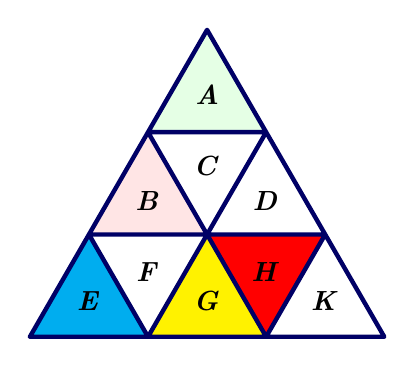
\begin{tikzpicture}[scale=1.5, line join=round, line cap=round]
			% Định nghĩa các điểm mốc cho tam giác đều lớn (cạnh là 3 đơn vị)
			% Tọa độ đỉnh (x, y) dựa trên sin(60) và cos(60)
			
			% Hàng 1 (Đỉnh)
			\coordinate (Top) at (1.5, 2.598);
			
			% Hàng 2
			\coordinate (L2_1) at (1, 1.732);
			\coordinate (L2_2) at (2, 1.732);
			
			% Hàng 3
			\coordinate (L3_1) at (0.5, 0.866);
			\coordinate (L3_2) at (1.5, 0.866);
			\coordinate (L3_3) at (2.5, 0.866);
			
			% Hàng 4 (Đáy)
			\coordinate (L4_1) at (0,0);
			\coordinate (L4_2) at (1,0);
			\coordinate (L4_3) at (2,0);
			\coordinate (L4_4) at (3,0);
			
			% --- Tô màu các tam giác nhỏ ---
			% A - Xanh lá nhạt
			\fill[green!10] (Top) -- (L2_1) -- (L2_2) -- cycle;
			% B - Hồng nhạt
			\fill[red!10] (L2_1) -- (L3_1) -- (L3_2) -- cycle;
			% E - Xanh dương
			\fill[cyan] (L3_1) -- (L4_1) -- (L4_2) -- cycle;
			% G - Vàng
			\fill[yellow] (L3_2) -- (L4_2) -- (L4_3) -- cycle;
			% H - Đỏ
			\fill[red] (L3_2) -- (L3_3) -- (L4_3) -- cycle;
			
			% --- Vẽ khung lưới tam giác ---
			\draw[blue!40!black, ultra thick] (Top) -- (L4_1) -- (L4_4) -- cycle (L2_1) -- (L2_2) (L3_1) -- (L3_3) (L2_1) -- (L3_2) -- (L2_2) (L3_1) -- (L4_2) -- (L3_2) -- (L4_3) -- (L3_3);
			
			% --- Gán nhãn chữ cái ---
			\node at (1.5, 2.05) {\textbf{\textit{A}}};
			\node at (1, 1.15) {\textbf{\textit{B}}};
			\node at (1.5, 1.45) {\textbf{\textit{C}}};
			\node at (2, 1.15) {\textbf{\textit{D}}};
			\node at (0.5, 0.3) {\textbf{\textit{E}}};
			\node at (1, 0.55) {\textbf{\textit{F}}};
			\node at (1.5, 0.3) {\textbf{\textit{G}}};
			\node at (2, 0.55) {\textbf{\textit{H}}};
			\node at (2.5, 0.3) {\textbf{\textit{K}}};
			
		\end{tikzpicture}
	}
	\par
	\shortans{0,13}
	\loigiai{
		Số phần tử của không gian mẫu là $n\left(\Omega\right) = 5^9$.\\
		Gọi $A$ là biến cố: \lq\lq Hai tam giác có chung cạnh được tô màu khác nhau\rq\rq.
		\begin{itemize}
			\item Số cách tô màu cho $6$ tam giác $B$, $C$, $D$, $H$, $G$, $F$ là $(5-1)\cdot (-1)^6 + (5-1)^6 = 4100$.
			\item Số cách tô màu cho $3$ tam giác $A$, $E$, $K$ là $4 \cdot 4 \cdot 4 = 64$.
		\end{itemize}
		Do đó $n(A)=262\,400$.\\
		Vậy xác suất cần tìm là
		$$\mathrm{P}(A) = \dfrac{n(A)}{n(\Omega)} \approx 0{,}13.$$
	}
\end{ex}
%%%=============EX_20=============%%%
\begin{ex}%[2D1H4-4]%[TDMT10]%[Nguyễn Thành Hậu]
	Cho một đa giác đều $(H)$ có $28$ đỉnh. Gọi $X$ là tập tất cả các tứ giác có $4$ đỉnh là đỉnh của $(H)$. Chọn ngẫu nhiên từ $X$ một tứ giác. Gọi $T$ là xác suất chọn ra một hình thang cân mà không phải hình chữ nhật. Hãy tính $1000T$ (\textit{làm tròn kết quả đến hàng đơn vị}).
	\par
	\shortans[0]{107}
	\loigiai{
		\begin{center}
			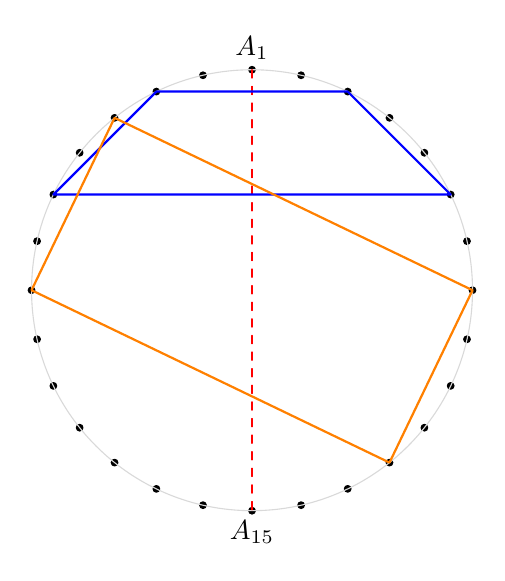
\begin{tikzpicture}[scale=0.8, line join=round, line cap=round]
				\def\R{3.5} 
				\def\n{28}  
				
				\foreach \i in {1,...,\n} {
					\coordinate (A\i) at ({90 - (\i-1)*360/\n}:\R);
					\filldraw (A\i) circle (1.5pt);
				}
				\draw[gray!30] (0,0) circle (\R);
				\draw[dashed, red] (A1) -- (A15); 
				\draw[thick, blue] (A3) -- (A6) -- (A24) -- (A27) -- cycle;
				\draw[thick, orange] (A8) -- (A12) -- (A22) -- (A26) -- cycle;
				
				\node[above] at (A1) {$A_1$};
				\node[below] at (A15) {$A_{15}$};
			\end{tikzpicture}
		\end{center}		
		\begin{itemize}
			\item \textbf{CÁCH 1:} Xét bài toán tổng quát đối với đa giác đều $2n$ đỉnh $A_{1}A_{2}\ldots A_{2n}$. Ta sẽ đếm số hình thang cân (kể cả hình chữ nhật) $A_{1}A_{i}A_{j}A_{k}$, trong đó $1<i<j<k\leq 2n$.\\
			Gọi $x$, $y$, $z$, $t$ lần lượt là số điểm nằm giữa các cặp điểm $(A_{1},A_{i})$, $(A_{i},A_{j})$, $(A_{j},A_{k})$, $(A_{k},A_{1})$ theo cùng một chiều nào đó. Ta có
			\[\heva{&x+y+z+t=2n-4\\ & x,y,z,t\in\mathbb{N}.}\]
			Tứ giác $A_{1}A_{i}A_{j}A_{k}$ là hình thang cân khi và chỉ khi $x=z$ hoặc $y=t$.\\
			Gọi $M=\{A_{1}A_{i}A_{j}A_{k}\mid x=z \}$ và $N=\{A_{1}A_{i}A_{j}A_{k}\mid y=t \}$. Ta sẽ tính số phần tử các tập $M$, $N$, $M\cap N$.\\
			Ta thấy số phần tử của tập $M$ là số cặp $(x,y,z,t)$ thỏa mãn hệ:
			\begin{equation}
				\heva{&x+y+z+t=2n-4\\ &x=z\\ &x,y,z,t\in\mathbb{N}}\Leftrightarrow \heva{&2x+y+t=2n-4\\ &x=z\\ &x,y,z,t\in\mathbb{N}.}\tag{*}
			\end{equation}
			Từ $2x+y+t=2n-4$ ta suy ra $0\le x\le n-2$. Với mỗi số tự nhiên $x$ thỏa mãn $0\le x\le n-2$ ta có $y+t=2n-4-2x$. Phương trình này có $2n-3-2x$ nghiệm $(y,t)$ là các số tự nhiên (vì với mỗi $0\le y\le 2n-4-2x$ thì có duy nhất một số tự nhiên $t$ thỏa mãn phương trình).\\
			Như vậy có tất cả $\displaystyle\sum_{x=0}^{n-2}(2n-3-2x)=(n-1)(2n-3)-2\cdot \dfrac{(n-2)(n-1)}{2}=(n-1)^{2}$ nghiệm $(x,y,z,t)$ của $(*)$. Do đó, $|M|=(n-1)^{2}$.\\
			Tương tự, $|N|=(n-1)^{2}$.\\
			Ta thấy số phần tử của tập $M\cap N$ là số nghiệm của hệ:
			\begin{equation}
				\heva{&x+y+z+t=2n-4\\ &x=z\\ &y=t\\ &x,y,z,t\in\mathbb{N}}\Leftrightarrow \heva{&2x+2y=2n-4\\ &x=z\\ &y=t\\ &x,y,z,t\in\mathbb{N}}\Leftrightarrow\heva{&x+y=n-2\\ &x=z\\ &y=t\\ &x,y,z,t\in\mathbb{N}.}\tag{**}
			\end{equation}
			Tương tự như trên, ta dễ dàng thấy rằng hệ $(**)$ có $n-1$ nghiệm. Vì thế $|M\cap N|=n-1$.\\
			Như vậy, số hình thang cân (kể cả hình chữ nhật) $A_{1}A_{i}A_{j}A_{k}$ là:
			\[|M\cup N|=|M|+|N|-|M\cap N|=2(n-1)^{2}-(n-1)=(n-1)(2n-3).\]
			Một cách tương tự, ta lần lượt đếm số hình thang cân có chứa đỉnh $A_{2}$, chứa đỉnh $A_{3}$, ..., chứa đỉnh $A_{2n}$ đều bằng $(n-1)(2n-3)$. Trong quá trình đếm như thế, một hình thang cân được đếm $4$ lần nên số hình thang cân có bốn đỉnh là bốn đỉnh của đa giác đều $2n$ cạnh là $\dfrac{2n(n-1)(2n-3)}{4}=\dfrac{n(n-1)(2n-3)}{2}$.\\
			Hơn nữa, số hình chữ nhật có đỉnh là đỉnh của đa giác đều $2n$ đỉnh bằng số cách chọn ra hai đường chéo đi qua tâm của đa giác đều và bằng $\mathrm{C}_{n}^{2}=\dfrac{n(n-1)}{2}$.\\
			Như vậy, số hình thang cân mà không là hình chữ nhật bằng $\dfrac{n(n-1)(2n-3)}{2}-\dfrac{n(n-1)}{2}=n(n-1)(n-2)$.\\
			Quay lại bài toán với $n=14$.\\
			Số cách chọn ra một tứ giác có bốn đỉnh là đỉnh của $(H)$ là $\mathrm{C}_{28}^{4}$. Số cách chọn ra một hình thang cân không phải hình chữ nhật là $14(14-1)(14-2)=2184$.\\
			Khi đó \[T=\dfrac{2184}{\mathrm{C}_{28}^{4}}\approx 0{,}1066\Rightarrow 1000T\approx 106{,}6\approx 107.\]
			\item \textbf{CÁCH 2:}		
			Xét bài toán tổng quát đối với đa giác đều $2n$ đỉnh $A_{1}A_{2}\ldots A_{2n}$ nội tiếp $(O)$. Khi đó, $A_{1}A_{n+1}$, $A_{2}A_{n+2}$, ..., $A_{n}A_{2n}$ là các đường kính của $(O)$.\\
			Gọi $X$ là số hình chữ nhật có các đỉnh là đỉnh của đa giác đều. Như trên, $X=\mathrm{C}_{n}^{2}$.\\
			Ta sẽ tính số hình thang cân có các đỉnh là đỉnh của đa giác đều.
			\begin{itemize}
				\item \textbf{Trường hợp 1.} Hình thang cân có trục đối xứng đi qua hai đỉnh của đa giác đều (chính là đường kính của $(O)$).
				\begin{center}
					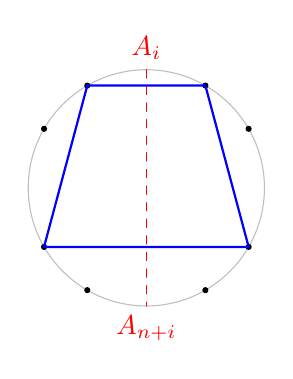
\begin{tikzpicture}[scale=0.6, line join=round, line cap=round]
						\def\R{2.5}
						\draw[gray!50] (0,0) circle (\R);
						\coordinate (A1) at (90:\R);
						\coordinate (An1) at (-90:\R);
						\draw[dashed, red] (A1) node[above]{$A_i$} -- (An1) node[below]{$A_{n+i}$};
						\foreach \ang in {30, 60, 120, 150, 210, 240, 300, 330} \filldraw (\ang:\R) circle (1.5pt);
						\draw[blue, thick] (60:\R) -- (120:\R) -- (210:\R) -- (330:\R) -- cycle;
					\end{tikzpicture}
				\end{center}
				Chọn một đường kính $A_{i}A_{n+i}$ của $(O)$ có $n$ cách. Với mỗi đường kính như thế có $n-1$ cặp điểm (hai điểm phân biệt) đối xứng nhau qua $A_{i}A_{n+i}$, số hình thang cân có trục đối xứng $A_{i}A_{n+i}$ bằng số cách chọn ra hai cặp điểm ở trên.\\ Vì thế, trường hợp này có $Y=n\mathrm{C}_{n-1}^{2}$ hình thang cân.
				
				\item \textbf{Trường hợp 2.} Hình thang cân có trục đối xứng không đi qua đỉnh của đa giác đều.
				\begin{center}
					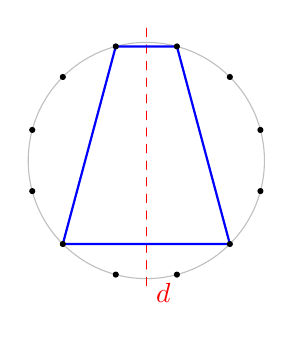
\begin{tikzpicture}[scale=0.6, line join=round, line cap=round]
						\def\R{2.5}
						\draw[gray!50] (0,0) circle (\R);
						\draw[dashed, red] (0,2.8) -- (0,-2.8) node[right]{$d$};
						\coordinate (M1) at (75:\R); \coordinate (M2) at (105:\R);
						\coordinate (M3) at (225:\R); \coordinate (M4) at (315:\R);
						\draw[blue, thick] (M1) -- (M2) -- (M3) -- (M4) -- cycle;						
						\foreach \ang in {15, 45, 75, 105, 135, 165, 195, 225, 255, 285, 315, 345} \filldraw (\ang:\R) circle (1.5pt);
					\end{tikzpicture}
				\end{center}
				Khi đó, trục đối xứng này phải là trung trực của một cạnh của đa giác đều. Có tất cả $n$ trục đối xứng như thế (vì trung trực của hai cạnh đối xứng nhau qua điểm $O$ trùng nhau). Chọn một trục đối xứng $d$ có $n$ cách. Khi đó, có $n$ cặp đỉnh của đa giác đều đối xứng qua $d$. Số hình thang có trục đối xứng $d$ chính bằng số cách chọn ra hai cặp điểm như trên.\\
				Vì thế, trường hợp này có $Z=n\mathrm{C}_{n}^{2}$ hình thang cân.
			\end{itemize}
			Với cách đếm như trên, mỗi hình chữ nhật sẽ được đếm $2$ lần (vì hình chữ nhật có hai trục đối xứng: một đi qua đỉnh và một không đi qua đỉnh) nên số hình thang cân bằng:
			\[R=Y+Z-X=n\mathrm{C}_{n-1}^{2}+n\mathrm{C}_{n}^{2}-\mathrm{C}_{n}^{2}.\]
			Số hình thang cân không phải hình chữ nhật là:
			\[S=R-X=n\mathrm{C}_{n-1}^{2}+n\mathrm{C}_{n}^{2}-2\mathrm{C}_{n}^{2}.\]
			Quay lại bài toán với $n=14$.\\
			Ta có $T=\dfrac{14\mathrm{C}_{13}^{2}+14\mathrm{C}_{14}^{2}-2\mathrm{C}_{14}^{2}}{\mathrm{C}_{28}^{4}}\approx 0{,}1066$, suy ra $1000T\approx 107$.
		\end{itemize}
	}
\end{ex}
%%%=============================%%%
\Closesolutionfile{ans}
\newpage
\indapan{12}{ans/ansTN-Dung}
\indapan[TF]{2}{ans/ansTN-DungSai}
\indapan[SA]{6}{ans/ansTN-DienKhuyet}
%%%%%%%%%%%%%%
%%nhãn kết thúc đề (để đếm số trang tự động mỗi đề)
\label{B\thedeso}